\section{Validation of the TLP-HMM}

\subsection{Model validation}

The response of the generator is tested in conditions as close as possible to the ISO 10605 standard \cite{iso10605}.
The generator is connected to a 2\textOmega{} load, itself connected to a 12 GHz (10 ps/sample point) oscilloscope with a 50\textOmega{} input impedance.
The setup (Fig. \ref{fig:injection_setup_validation}) has the same loading impedance than the standard measurement target \cite{iso10605, iec61000-4-2}.

\begin{figure}[!h]
  \centering
  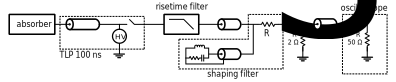
\includegraphics[width=0.9\textwidth]{src/5/figures/validation_injection_setup.pdf}
  \caption{Injection setup for validating the generator}
  \label{fig:injection_setup_validation}
\end{figure}

The measured and simulated waveforms are given in Fig. \ref{fig:tlp_hmm_waveforms}.
Measured currents at 30ns and 60ns are within the 30\% tolerance of the standard (see Table \ref{tab:mes-sim-std-currents}).
The measured peak current is a bit lower (110 mA short of minimum margin) than standard value.
This is easily corrected on the TLP by adding a small positive offset to the charging voltage.

\begin{figure}[!h]
  \centering
  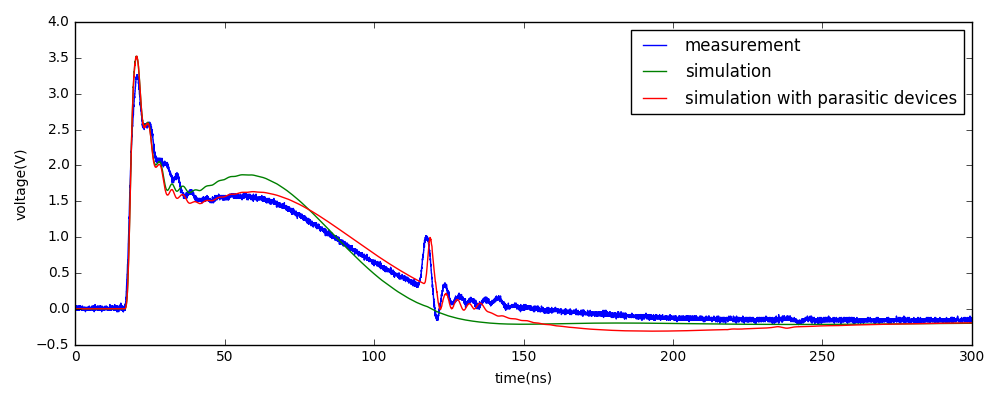
\includegraphics[width=0.95\textwidth]{src/5/figures/tlp_hmm_waveforms.png}
  \caption{Measurement versus simulation of a 250V TLP-HMM (equivalent 1kV HMM) on 2\textOmega{}}
  \label{fig:tlp_hmm_waveforms}
\end{figure}

\begin{table}[!h]
\centering
\begin{tabular}{@{}llll@{}}
\toprule
         & Standard (A)    & Measured (A)  & Simulated (A) \\ \midrule
peak     & 3.75 \pm 0.375  & 3.26          & 3.52 \\
30 ns    & 2 \pm 0.6       & 1.54          & 1.8  \\
60 ns    & 1 \pm 0.3       & 1.18          & 1.32 \\ \bottomrule
\end{tabular}
\caption{Measured and simulated currents versus standardized values}
\label{tab:mes-sim-std-currents}
\end{table}

% Analyse the curve
Overall, simulation and measurement correlate quite well.
There is a small difference for the slopes between 40ns and 150ns.
Investigation showed this difference comes from the shaping filter, and the inductances in particular.
Their frequency behavior is not as good as expected.
Having four inductances in parallel increases further this issue.
In the current shaping filter configuration, the parasitic capacitance of each inductor are in parallel.
They add up together, leading to a degraded frequency behavior.
For the next iteration of the shaping filter, a single RF inductor should be used instead.
The shaping filter model can be corrected by connecting in parallel a total parasitic capacitance of 2nF in series with a 15\textOmega{} parasitic resistor.

\begin{figure}[!h]
  \centering
  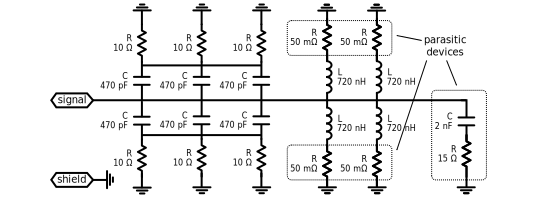
\includegraphics[width=0.8\textwidth]{src/5/figures/shaping_filter_schematic_parasitics.pdf}
  \caption{shaping-filter schematic with parasitics}
  \label{fig:shaping_filter_schematic_parasitics}
\end{figure}

The glitch visible at approximately 120 ns is due to the absorber, because of two different parasitic devices.
At the beginning of the TLP pulse, the parasitic capacitance between signal and ground is charged.
Using the simulation, it is estimated at 20 pF.
Its sudden discharge at the end of the TLP pulse causes the short voltage and current increase observed at 120 ns.
The parasitic series inductance of the three 2.2nF capacitors and the 50\textOmega{} resistor (Fig. \ref{fig:absorber_schematic_parasitics}) is responsible afterward for the small oscillation observed between 120 ns to 150 ns.
This issue should be fixed in the next iteration of the absorber by building the absorber on a dedicated PCB with 50\textOmega{} lines.
Guarantying matching along the path should eliminate this ringing oscillation.

\begin{figure}[!h]
  \centering
  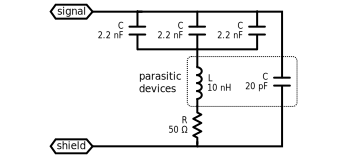
\includegraphics[width=0.5\textwidth]{src/5/figures/absorber_schematic_parasitics.pdf}
  \caption{absorber schematic with parasitics}
  \label{fig:absorber_schematic_parasitics}
\end{figure}

% TODO: Do next ?
% Afterwards, resistive loads of 2 10 and 0 are tested
% The first two loads are simply constituted of several resistors in parallel.
% The oscilloscope input impedance is used for the 50  load.
% In this case, reflections are eliminated by the matched load and the waveform is less disturbed.

% For 2 and 10, the measurements (Fig. 16 & 17) are quite noisy because of reflections.
% Despite that, it is interesting to observe that overall the amplitudes match well.
% The differences come mostly from parasitic devices not taken into account in those simulation.
%TODO: Waveforms 2ohm, 10ohm, 50ohms


\subsection{Comparison with an ESD Gun}

% Introduce how generators are usually tested against ESD gun
A generally adopted procedure to compare any ESD generator to another is to destroy ESD protections and compare the failure levels.
The TLP-HMM is compared to a real standardized HMM generator following this procedure.
The failure criteria is a sudden increase in the leakage current of the tested ESD protection after a pulse injection.

% Detail the devices that are going to be tested
A set of ten different ESD protections, of different size, on-resistance, structure and failure levels are stressed with both generators.
Five samples are tested for each structure and generator, to ensure the failure levels do not exhibit large variations.
Table \ref{tab:esd-protections} gives the on-resistance for each tested device.
%This property is employed later to build a correlation method.

\begin{table}[!h]
\centering
\begin{tabular}{@{}lllllllllll@{}}
\toprule
Structure                          & A    & B    & C     & D    \\ \midrule
R\textsubscript{ON} (\textOmega{}) & 6.2  & 2.85 & 9.72  & 13.3 \\
\end{tabular}
\caption{Tested ESD protection set}
\label{tab:esd-protections}
\end{table}

% Test results & limitations
Testing results are summarized in Table \ref{tab:esd-protections}.
Unfortunately, the result set is too small to draw a clear conclusion.
It was discovered that the TLP-HMM is not able to deliver enough current to break structure E and above.
The TLP-HMM relies on a regular TLP, whose high-voltage DC supply is limited to 1kV.
On a true HMM generator, the supply are generally able to reach 15kV charging voltage and beyond.
A TLP rarely requires DC supplies able to reach above 1kV, because the output impedance is lower than HMM.
For a given charging voltage, a TLP will deliver a much larger amount of current than an HMM generator.

\begin{table}[!h]
\centering
\begin{tabular}{@{}lllllllllll@{}}
\toprule
Structure   & A     & B     & C      & D    & E    & F    & G     & H    & I     & J      \\ \midrule
TLP-HMM (V) & 640   & 700   & 890    & 860  & -    & -    & -     & -    & -     & -      \\
HMM     (V) & 1250  & 1250  & 1500   & 1500 & 6500 & 5000 & 13000 & 9500 & 20000 & 145000 \\
\end{tabular}
\caption{Testing results - failure levels per ESD protection}
\label{tab:esd-protections}
\end{table}

\subsection{Correlation between TLP and HMM}

% Correlation method principle orrelation results
%TODO: Review
Based on those preliminary results, a correlation method was built between TLP failure levels and HMM failure levels.
It exploits the fact that the TLP-HMM is at its core a TLP and has a similar behavior to an HMM generator.
It was published in \cite{my-publi-tlp-hmm}.
Characterize each generator, and build a Thevenin equivalent circuit with resistor and DC voltage.
DC voltage is charging voltage (command set on the generator), and resistor is extracted from characterization
ESD protection is represented by its on-resistance.
Total equivalent circuit is just a DC source with two resistors in series, and is given in Fig \ref{fig:simple_equivalent_circuit}.

%TODO: Equivalent circuit
\begin{figure}[!h]
  \centering
  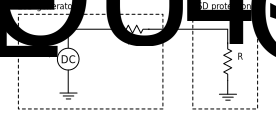
\includegraphics[width=0.5\textwidth]{src/5/figures/equivalent_circuit.pdf}
  \caption{Simple equivalent circuit for the correlation}
  \label{fig:simple_equivalent_circuit}
\end{figure}

It is found in the article that for both TLP and HMM, DC source voltage and resistances are different.
But the failure current found with this method is extremely close for both generators, for each of the 10 tested structures.
Ultimately, a prediction method is built from this result.
It requires the TLP failure voltage, and the ESD-on resistance, to predict the HMM failing voltage.
Both values are easily obtained from a TLP characterization.

%TODO: Plot of correlation method
\begin{figure}[!h]
  \centering
  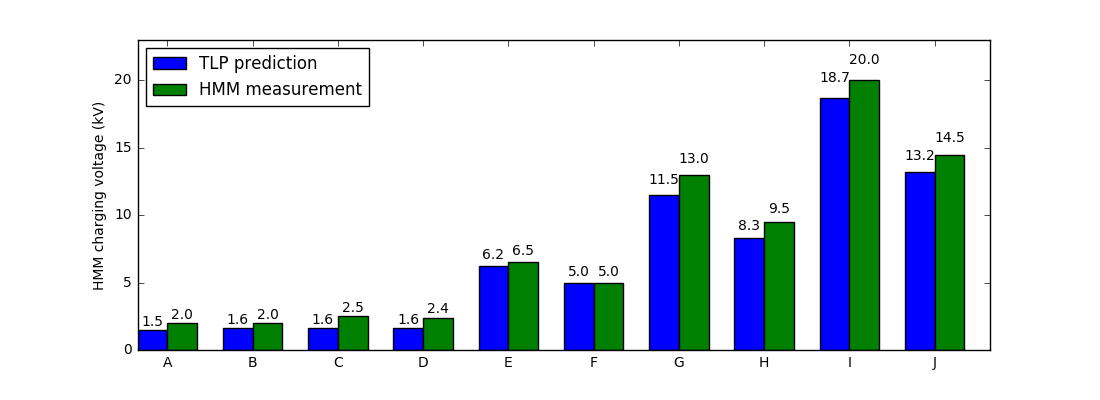
\includegraphics[width=0.5\textwidth]{src/5/figures/correlation_results.png}
  \caption{TLP-predicted versus HMM-measured failure levels }
  \label{fig:predicted_vs_measured_levels}
\end{figure}

Fig. \ref{fig:predicted_vs_measured_levels} shows the results of this prediction method on the same set of 10 ESD protections.
Extremely good correlation show that this method could have great potential.
